\procTitle{Опыт определения  предмета охраны археологической стоянки <<поселение Бугурчан II--I~тыс.~до~н.~э. (четыре~жилища)>>}
\procAuthor{Зеленская~А.\,Ю.}
\procEmail{zelenskaya@neisri.ru}
\procOrganization{СВКНИИ ДВО РАН} \procCity{Магадан}

\makeProcTitleRazdel
\index{z@Зеленская~А.\,Ю.}

Для постановки на учёт и охрану объектов культурного наследия (в~т.~ч. объектов археологического наследия) в органах исполнительной власти регионов, помимо проведения полевых и камеральных работ, необходимо определить, изучить и описать предмет его охраны. \textbf{Предмет охраны}~--- это особенности объекта культурного наследия, которые представляют его культурную ценность и служат основанием для постановки этого объекта на~государственный учёт.

С правовой точки зрения, необходимость определения предмета охраны, закреплена в Федеральном законе от 25 июня 2002~года 73-ФЗ <<Об объектах культурного наследия (памятниках истории и культуры) народов Российской Федерации>> (статья 15). Изданием приказов об утверждении предметов охраны объектов культурного наследия (далее~--- ОКН) Магаданской области занимается отдел по охране ОКН при Правительстве Магаданской области.

До недавнего времени Отдел по охране ОКН издавал приказы об утверждении предметов охраны только для памятников архитектуры. Определение предмета охраны таких объектов является процессом, зачастую, однозначным и объективным. Например, предметом охраны любого исторического здания, является его конструкция и внутренне убранство (элементы интерьера/экстерьера архитектурного сооружения). Но определение предмета охраны объекта археологического наследия (далее~--- ОАН) сопряжено с рядом трудностей, а именно: 1)~необходимостью актуального мониторинга состояния ОАН и 2)~точным определением границ распространения культурного слоя (который является одним из главных элементов предмета охраны), из чего сразу возникает парадокс~--- изучая культурный слой, мы его одновременно и уничтожаем.

 По заданию отдела по охране ОКН Правительства Магаданской области в~2019~г., сотрудниками лаборатории истории и экономики СВКНИИ ДВО РАН~--- ведущим научным сотрудником, к.\,и.\,н. Слободиным~С.~Б. и младшими научным сотрудником Зеленской~А.~Ю. были выполнены работы по~определению предмета охраны для стоянки-поселения Бугурчан (стоянка находится на~Государственной охране решением исполнительного комитета Магаданского облсовета народных депутатов от 29.04.1974 №~174).

Ранее, в~2017~г., этими же сотрудниками был проведён мониторинг данной стоянки [2], в~результате которого был составлен топографический план, определены границы ОАН посредством заложения шурфов и зачисток, а также локализованы на местности ландшафтные элементы стоянки (местонахождения полууглубленных жилищ).

В процессе работы над проектом был выполнен анализ всей имеющейся учётной документации, публикаций об объекте археологического наследия, выполнен сбор и анализ результатов археологических обследований на~территории расположения объекта археологического наследия (материалы архивного фонда Магаданского областного краеведческого музея и научно-отраслевого архива Института археологии РАН) и результатов археологических работ 2017~г.

Стоянка-поселение Бугурчан находится на полуострове Кони, на южном берегу залива Одян. Она располагается на высокой морской террасе, протянувшейся по~левому берегу р.~Богурчан на территории бывшего пос.~Бугурчан.

Первые сведения о стоянке поступили в Магаданский областной краеведческий музей (далее~--- МОКМ) в~1939~г. от эвена-охотника И.~Бабцева, который сообщал о <<коряцких ямах>> в~устье р.~Богурчан [3]. В~1955~г. археологический отряд Якутского филиала АН СССР и МОКМ (рук. Г.~А.~Пытляков и А.~В.~Беляева) провёл обследование стоянки, представленной тогда выраженными в рельефе западинами округлых в пла­не полуподземных жилищ [4; 5]. В ходе обследования было обнаружено шесть округлых в плане полуподземных жилищ [4, Л.~54]. Одно располагалось у моря, на первой надпойменной террасе р.~Богурчан, вблизи пирса и рыбзавода и было полностью уничтожено морским прибоем, еще 5 жилищ найдено на террасе, где располагался поселок [2, С.~7; 1, С.~144]. Материалы раскопок опубликованы Р.~С.~Васильевским [1, С.~66-69].

При проведении мониторинга в 2017~г. локализовать на местности указанные Г.~А.~Пытляковым жилища не удалось по причине того, что жилища №~1--4, были, очевидно, разрушены при строительстве посёлка и нивелированы с поверхностью террасы хозяйственной деятельностью. Но культурный слой, как выяснилось, сохранился. Судя по разрушенным остаткам пирса и рыбозавода заливаемых морем, и по сообщению живущих там сторожил, морская терраса, где расположена стоянка, была разрушена морем примерно на 10--15~м, так, что жилища №~5 и 6 к настоящему времени полностью смыты морем.
Заложенные по краю террасы и в ее глубине в ходе мониторинга 2017~г. 6 зачисток и шурфов подтвердили наличие на террасе сохранившегося от древнего поселения культурного слоя с находками каменных, костяных орудий и керамики.

Суммируя полученные данные было определено, что мощность культурного слоя стоянки варьируется от 10 до 40 см. Сохранность культурного слоя стоянки средняя, что связано с современной антропогенной деятельностью. Площадь распространения культурного слоя прослеживается от зачистки у берегового обрыва вглубь по террасе на юг на расстояние до 120--130~м. Археологические находки характерны для древнекорякской культуры I--II~тыс.~н.~э.

В соответствии с контекстом изученного археологического материала был описан предмет охраны поселения. Данный археологический объект обладает историко-культурной ценностью, являясь источником информации развитии культуры населения Охотского побережья в позднем голоцене, в~эпоху палеометалла. Стоянка представляет научный интерес в перспективе построения культурно-хронологической схемы развития культур с приморской адаптацией, характеристике культурной принадлежности древних обитателей, техники каменного производства и хозяйственной деятельности. Памятник перспективен для дальнейшего научного изучения. Сохранению подлежат культурные остатки, залегающие на глубине до 0,4~м. Площадь территории объекта и, соответственно, распространения отложений с~культурным слоем, уточнена в результате геодезических работ и составляет 18\,891~м$^2$.

Таким образом, предметом охраны объекта культурного (археологического) наследия федерального значения <<Поселение Бугурчан II--I~тыс. до~н.~э.>> были определены следующие элементы:

1. Территория ОАН в пределах утверждённых границ на общей площади  18\,891~м$^2$ (см.~рис.).

\begin{figure}[h!]
  \begin{center}
    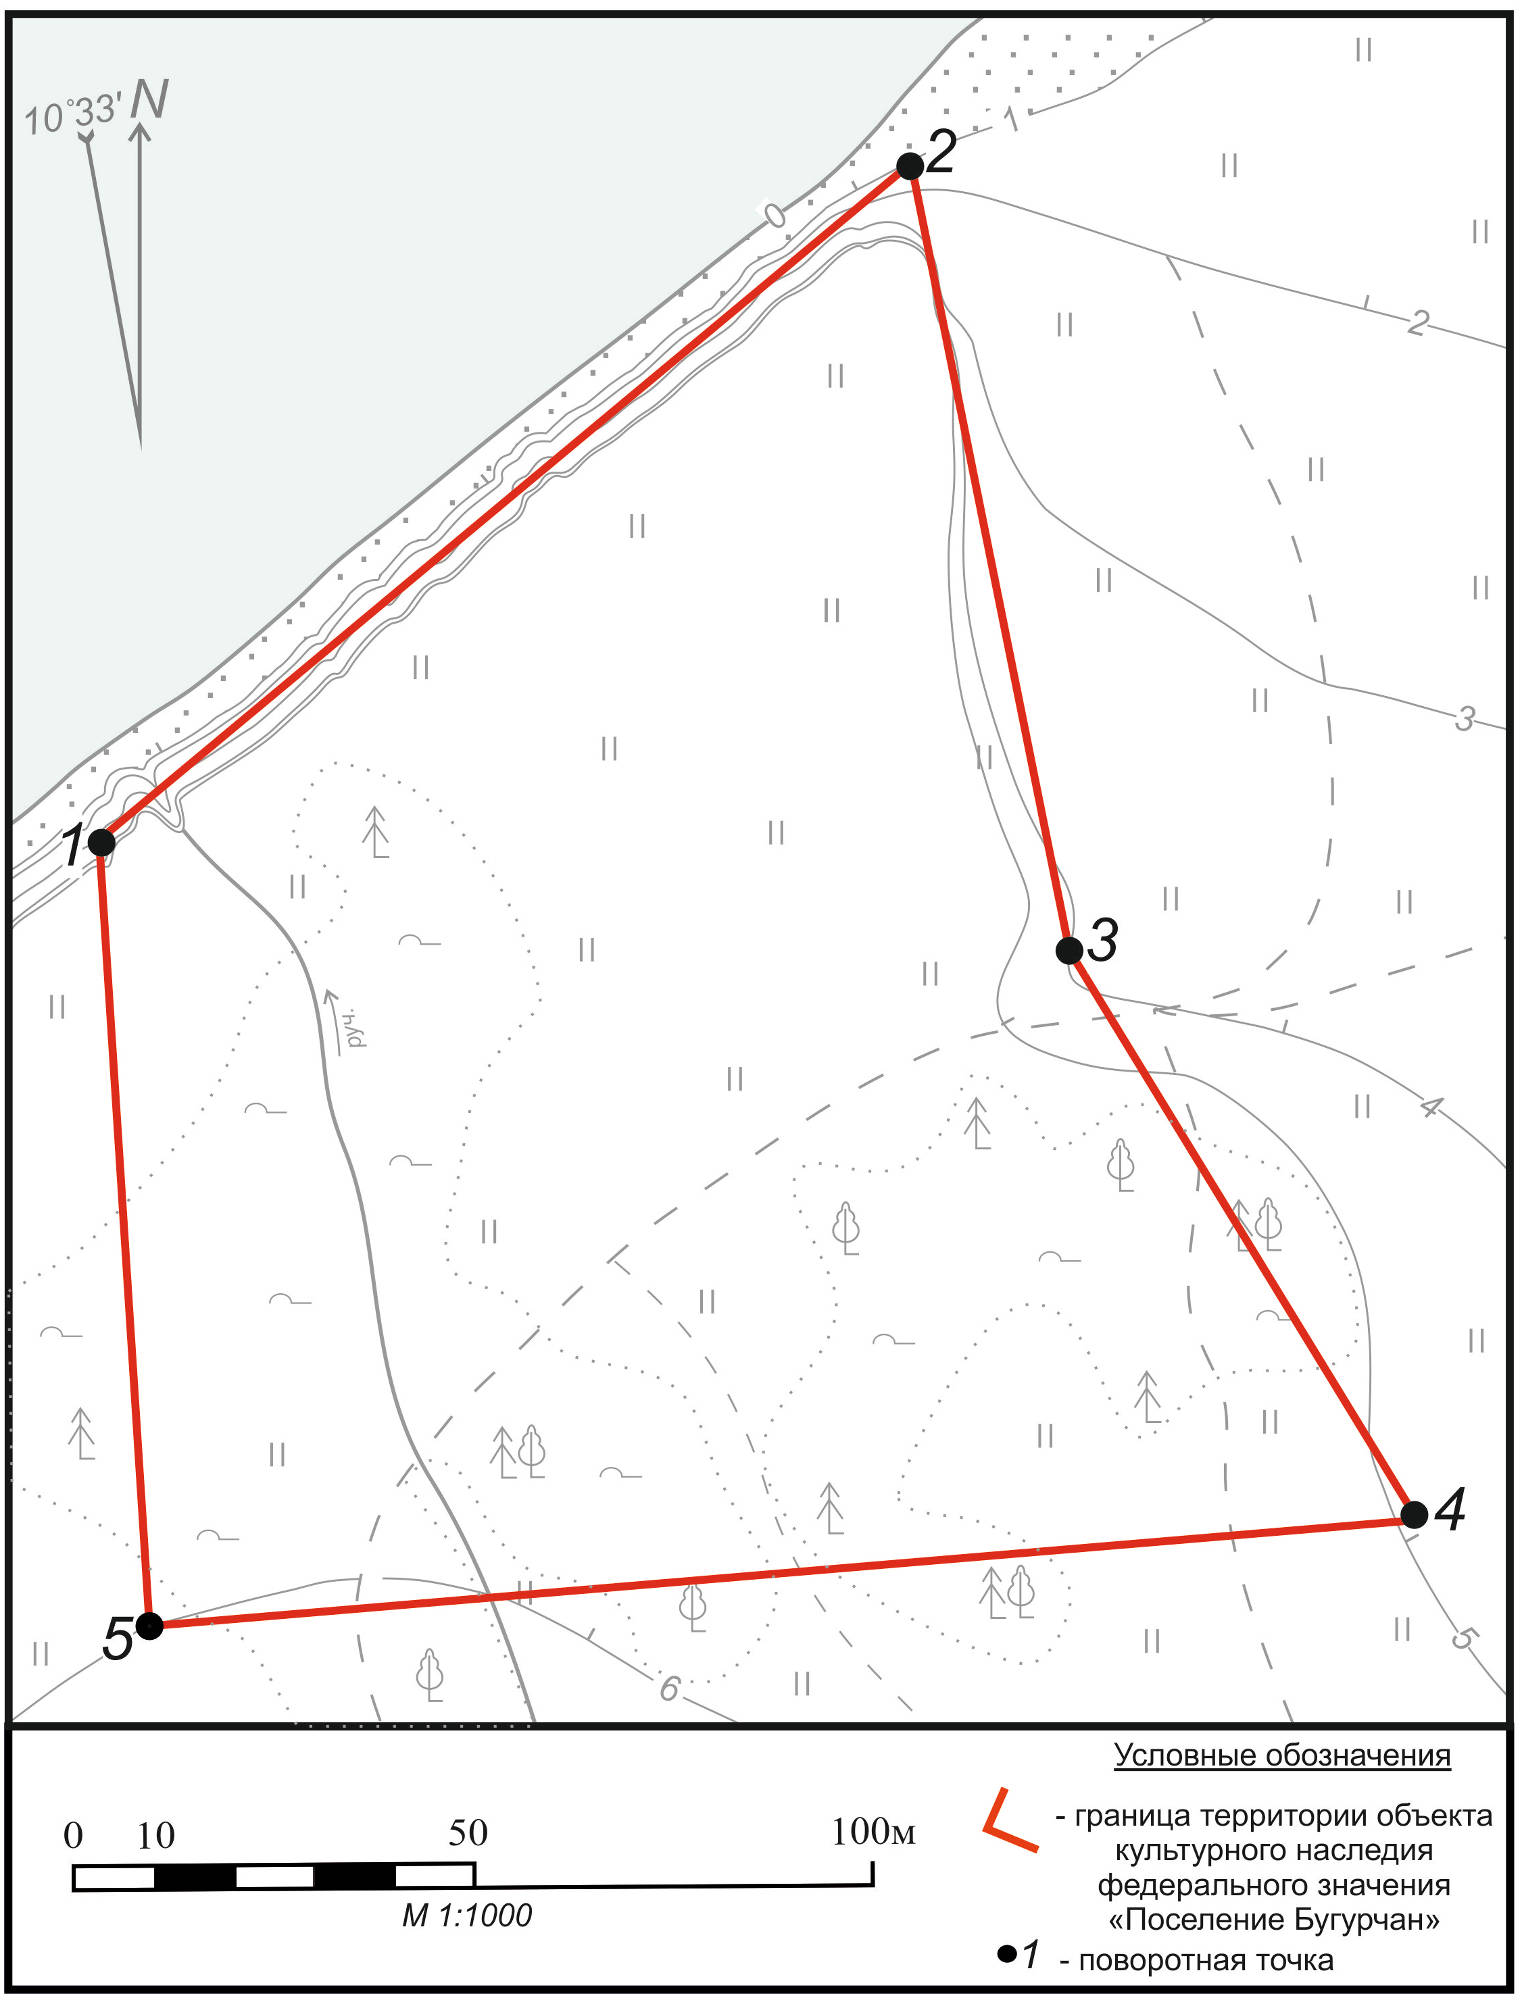
\includegraphics[width=0.8\textwidth]{authors/zelenskay.jpg}
  \end{center}
  \caption*{\textbf{Схема расположения границы территории ОКН <<Поселение Бугурчан>>}}
  \label{fig:zelenskay}
\end{figure}


2. Культурный слой, несущий в себе остатки жизнедеятельности древнего человека, частично или полностью скрытый под землёй (представлен основанием тёмно-коричневой гумусированной супеси в сочетании с кровлей рыжего суглинка или бурой супеси с линзами углистости на глубине от 10 до 40~см от~дневной поверхности.

3. Археологические недвижимые и движимые объекты, содержащиеся на современной дневной поверхности ОАН, в составе грунтовых напластований (конструкции и сооружения, антропологические и остеологические материалы, археологические предметы, следы жизнедеятельности древнего человека): миниатюрное тесло или нож треугольной формы из кремнистой породы; наконечник стрелы треугольной формы из кремнистого сланца с прямыми длинными сто­ронами и небольшой овальной выемкой в основании; массивный наконечник копья или китового гарпуна из тёмного кварцита листовидной формы с черешковым насадом; два продолговатых тесла из чёрного кремнистого сланца с острым обушком, выпуклым широким рабочим краем; два скребка; три грузила для сетей; шесть небольших аморфных нуклеусов а также фрагменты керамики с ложнотекстильным оттиском (материалы раскопок 1956~г.). Отщепы, каменное тесло, костяное орудие и керамика с налепными валиками, отогнутым венчиком, и вафельным отпечатком (материалы мониторинга 2017~г.).

Материалы раскопок стоянки-поселения Бугурчан хранятся в Магаданском областном краеведческом музее и Музее естественной истории СВКНИИ ДВО РАН.

4. Видимые на поверхности сооружения в виде котлованов жилищ и~объектов хозяйственного назначения. В 1955~г. археологический отряд Магаданского краеведческого музея под руководством Пытлякова~Г.~А., в ходе археологической разведки в устье р.~Богурчан, выявил шесть округлых полуподземных жилищ, выраженных в рельефе западинами. В 1956~г. была осуществлена полная раскопка жилища №~1.

В ходе мониторинга 2017~г. выяснилось, что жилища № 5 и 6, которые располагались на краю береговой террасы, были уничтожены морским прибоем. Локализовать на местности указанные Г.~А.~Пытляковым жилища удалось лишь приблизительно по архивным данным, т.~к. видимые западины в рельефе были нивелированы в ходе хозяйственной деятельности по~террасе. Вместе с тем, заложенные на стоянке-поселении стратиграфические разрезы показали наличие сохранившегося культурного слоя, не затронутого в процессе снятия верхнего почвенного горизонта. Таким образом, предметом охраны в данном случае, выступают снивелированные западины жилищ №~1--4.

5. Ландшафтно-пространственное и видовое восприятие участка в границах территории ОАН. В связи  с тем, что объект культурного наследия поселение Бугурчан расположен за пределами градостроительной среды, его ландшафтно-пространственное восприятие строиться на основе анализа физико-географической обстановки. Композиция стоянки, расположенной в природной среде, подчинена её своеобразию.

Стоянка-поселение Бугурчан находится на пол-ве Кони, в~зал.~Одян, на~его южном берегу, на 2-й надпойменной террасе слева от устья р.~Богурчан, где ранее располагался посёлок Бугурчан. На левом берегу р.~Богурчан выделяются первая и вторая надпойменные террасы. Первая надпойменная терраса имеет чётко выраженный тыловой шов на стыке со второй надпойменной террасой, на которой и расположена стоянка Бугурчан. В районе берега моря сочленение террас образует своеобразную <<стрелку>>, с которой открывается хороший обзор как в обе стороны по берегу моря, так и~вверх по долине р.~Богурчан. B 400--450~м от её устья, в долине р.~Богурчан происходит нивелировка первой и второй террас в одну.

Высокая, пологая, с небольшим подъемом вторая надпойменная терраса на левом берегу р.~Богурчан протянулась от ее устья к западу, вдоль берега моря и к югу, по долине р.~Богурчан на несколько сотен метров. Тыловой шов визуально не выделяется. Береговой уступ террасы со стороны моря обращён к северу (имеет северную экспозицию), обрывист, но хорошо задернован, высотой до 5~м. Подвергается разрушению только в сильные шторма. В~120~м от её края (от <<стрелки>>) в море впадает небольшой ручей, который, видимо, служил источником питьевой воды для древнего населения, обитавшего на этой террасе. По левому берегу ручья отмечены заболоченные участки террасы.

Вторая надпойменная терраса, на которой локализована стоянка Бугурчан, представляет собой открытую пространственную единицу ландшафта. Конфигурация зрительных барьеров сложена из низкорослого древостоя террасы, локализованного в её обрамлении (с восточной и южной стороны) и хозяйственных построек. Существующие постройки ввиду своих малых габаритов (не более 8~м в~высоту) и разреженности, не препятствуют визуальному изучению участка расположения ОКН. Таким образом, обзор на~стоянку не имеет ограничений.

Наиболее оптимальной зоной восприятия памятника является приустьевая часть террасы р.~Богурчан, точка обзора~--- в направлении восток-запад, и подножие сопки на юго-востоке, точка обзора~--- в направлении юго-запад~--- северо-восток. Таким образом, предметом охраны выступает обеспечение визуального восприятия объекта культурного наследия в его исторической и природной среде (запрещение перекрытия основных видовых точек и панорам, нарушающих визуальное восприятие объекта культурного наследия в его исторической среде).

Подводя итог проделанной работе по определению предмета охраны ОАН стоянки-поселения Бугурчан, необходимо отметить важность предварительно проведённых полевых работ, которые позволили определить утерянные для охраны элементы стоянки (разрушенные морским прибоем, жилища №~5 и 6), а также произвести поиск сохранившегося культурного слоя. Таким образом, все элементы и качественные особенности археологической стоянки, зафиксированные при проведении мониторинга в 2017~г., были поставлены на охрану Приказом Отдела по охране объектов культурного наследия Правительства Магаданской области №~23 от 11.12.2019.
\clearpage
\begin{thebibliography}{99}

\bibitem{}\BibAuthor{Васильевский~Р.~С.} Происхождение и древняя культура коряков.~--- Новосибирск, 1971.~--- 252~с.

\bibitem{}\BibAuthor{Пытляков~Г.~А., Беляева~А.~В.} Археологические работы на Охотском побережье //  Краеведческие записки.~--- Магадан~:МОКМ, 1957.~--- Вып.~I.~--- С.~5--11.

\textbf{Архивые источники}

\bibitem{}\BibAuthor{Зеленская~А.~Ю.} Научный отчёт по теме <<Археологические исследования в~Омсукчанском, Тенькинском, Ольском, Хасынском городских округах и~в~муниципальном образовании ,,\,г.~Магадан\,‘‘ Магаданской области в 2017~г. В~2-х~томах>> // Научно-отраслевой архив ИА~РАН. Ф.~1.
\bibitem{}\BibAuthor{Пытляков~Г.~А.} Отчёт и материалы предварительного исследования археологических памятников разведывательным отрядом Якутского филиала АН~СССР и Магаданского музея // МОКМ. Оп.~1. Д.~235.
\bibitem{}\BibAuthor{Пытляков~Г.~А.} Отчёт о проделанной работе археологическим разведывательным отрядом в верховьях реки Индигирки и на побережье Охотского моря летом 1955 г. // Архив ИА РАН. Ф.~1. Р.~1. №~1100. 94 л.



\end{thebibliography}
